\documentclass{beamer}
\usepackage{beamerthemeshadow}
\usepackage{graphicx}
\usepackage{xcolor}
\usepackage[utf8]{inputenc}
\usepackage{hyperref}
\usepackage{caption}
\usepackage[flushleft]{threeparttable}
\usepackage[english, serbian]{babel}
\usepackage{subfigure}
\usepackage{blindtext}
\definecolor{royalblue}{RGB}{65, 105, 225}
\setbeamercolor{structure}{fg=royalblue}
\captionsetup[figure]{labelformat=empty}
\captionsetup[table]{labelformat=empty}


\def\d{{\fontencoding{T1}\selectfont\đ}}
\def\D{{\fontencoding{T1}\selectfont\Đ}}


\title{Tehničko i naučno pisanje}
\subtitle{-- 3D štampa --}
\author{Nevena Miletić\and Matija Todorović\\ \and Relja Gajić \and Đorđe Sajić}
\institute{Matematički fakultet\\Univerzitet u Beogradu}
\date{
	\footnotesize{Beograd, 2022.}	
}

\begin{document}
\begin{frame}
	\thispagestyle{empty}
	\titlepage
\end{frame}

\addtocounter{framenumber}{-1}

\begin{frame}[fragile]\frametitle{Literatura}
	\begin{itemize}
		\item Zasnovano na seminarskom radu "3D štampa - Nevena Miletić, Matija Todorović, Relja Gajić i Đorđe Sajić ", koji se može naći na sledećem linku:
		(\url{https://github.com/NevenaMileticc/19_TNP2022/blob/main/19_MileticTodorovicGajicSajic.pdf })
	\end{itemize}
\end{frame}

\begin{frame}
	\frametitle{Pregled} 
	\tableofcontents[] 
\end{frame}
\section{3D štampa}
\subsection{Uvod}

\begin{frame}[fragile]\frametitle{Uvod - Šta je 3D štampa?}
	\begin{itemize}
	    \item 3D štampa je moderna tehnologija proizvodnje trodimenzionalnih objekata. 
            \item Omogućava izradu objekta od više različitih materijala, različitih mehaničkih i fizičkih svojstava u jedinstvenom procesu. 
            \item Popularni naziv tehnologije 3D štampa nije potpuno tačan, odgovarajući termin prema ISO standardu je aditivna manufaktura. 
            \item Pored aditivne razlikujemo i pojam subtraktivne manufakture.
Termin koji objedinjuje termine 3D štampe i aditivne manufakture je AM tehnologije. 
	\end{itemize}
\end{frame}

\subsection{Istorija razvoja 3D štampe}

\begin{frame}[fragile]\frametitle{Istorija razvoja 3D štampe}

\begin{table}[h!]
\begin{center}
\caption{Najbitnije godine u razvoju 3D štampe}
\begin{tabular}{|c|l|} \hline
\textbf{Kada se dogodilo?}& \textbf{\ Šta se dogodilo?}\\ \hline
80-ih godina prošlog veka &Prve ideje o aditivnoj manufakturi\\ \hline
1981. &Kodama je izmislio dva AM metoda\\ \hline
1984. &Hull dizajnira prvi 3D štampač\\ \hline
1986. &Hull štampa prvi predmet\\ \hline
1989. &Crump je izumeo FDM tehnologiju\\ \hline
1989. &Carl Deckard razvio je SLS\\ \hline
\end{tabular}
\label{tab:tabela1}
\end{center}
\end{table}
\end{frame}


\subsection{Tehnike 3D štampe}

\begin{frame}[fragile]\frametitle{Tehnike 3D štampe}
	\begin{itemize}
    \item Po tehnici 3D štampanja možemo razlikovati:
    \begin{itemize}
        \item Inkjet
        \item  Fused Deposition Modeling (FDM)
        \item Stereolitografija
        \item Selective laser sintering (SLS)
        \item Laminated Object Manufacturing (LOM)
        
    \end{itemize}
\begin{figure}[!tbp]
  \centering
  \subfloat {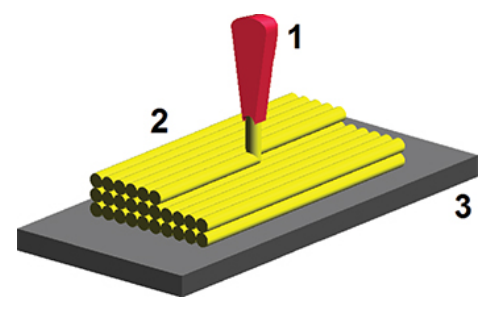
\includegraphics[width=0.3\textwidth]{fdm.PNG}\label{fig:f1}}
  \hfill
  \subfloat  {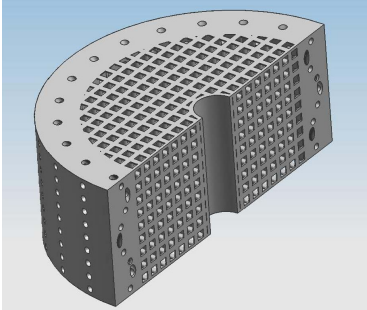
\includegraphics[width=0.3\textwidth]{sls.PNG}\label{fig:f2}}
  \hfill
  \subfloat  {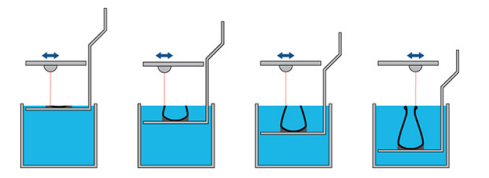
\includegraphics[width=0.3\textwidth]{stereolitografija.PNG}\label{fig:f3}}
  \label{Slika 1}
    \caption{\scriptsize{Slika1:Tehnike 3D štampe}}
    \end{figure}
\end{itemize}
\end{frame}
\subsection{Inkjet}


\subsection{FDM}

\begin{frame}[fragile]\frametitle{Odlike }
	\begin{itemize}	
		\item \textbf{Inkjet} - model se pravi jedan po jedan sloj, omogućava štampanje prototipa u punoj boji
		\item \textbf{FDM} - objekat se gradi nanošenjem rastopljenog termoplastičnog polimera na unapred određenu putanju sloj po sloj. 
            \item \textbf{Stereolitografija} - modeli se proizvode tako što zrak UV svetla prelazi preko bazena sa fotoosetljivom tečnošću
            \item \textbf{SLS} - UV svetlo je zamenjeno laserom, a bazen sa fotopolimerom sa praškastim materijalom
            \item \textbf{LOM} - Koriste se slojevi materijala, papira ili plastike, isečeni laserom
            
	\end{itemize}

\end{frame}


%\subsection{Stereolitografija}
%\begin{frame}[fragile]\frametitle{Stereolitografija}
%\begin{itemize}

%\end{itemize}

%\end{frame}


\subsection{Primena}

\begin{frame}[fragile]\frametitle{Primena}
	\begin{itemize}
	    \item \textbf{Medicina} - 3D štampanje se koristi za štampanje novih, zdravih tkiva.
	    \item \textbf{Prototipi} - Omogućava štampanje prototipa u kratkom vremenskom roku.
	    \item \textbf{Vojna primena} - Koristi se za štampanje delova za oružje.
	    \item \textbf{Izrada obuće i odeće} - Za štampanje pojedinih delova odevnih predmeta (npr. kramponi za kopačke).  
	\end{itemize}
\end{frame}

\section{Zaključak}

\begin{frame}[fragile]\frametitle{Zaključak}
	\begin{itemize}
	\item Zahvaljujući 3D štampi se:
\begin{itemize}
\item skraćuje vreme dolaska proizvoda na tržište
\item skraćuje vreme razvoja proizvoda uz snižavanje troškova
\end{itemize}
	\end{itemize}
\end{frame}

\end{document}